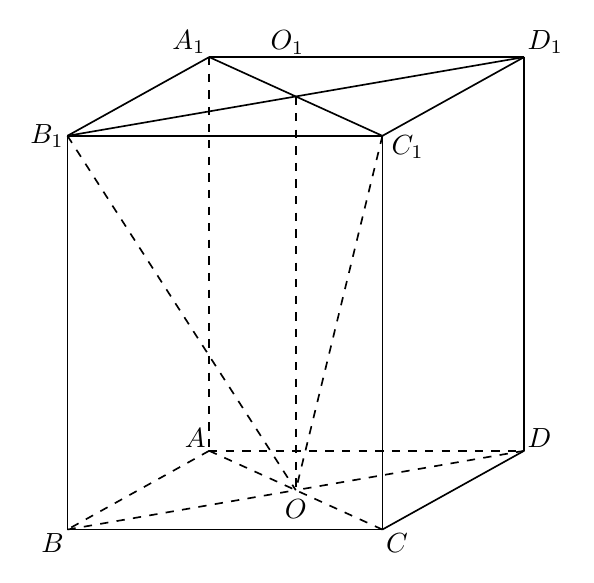
\begin{tikzpicture}[x=1cm,y=1cm,line width=.6pt]
\tikzset{lbl/.style={font=\normalsize,inner sep=1pt,fill=none}}
\coordinate (B) at (0,0);
\coordinate (C) at (4,0);
\coordinate (D) at (5.8,1.0);
\coordinate (A) at (1.8,1.0);
\coordinate (O) at (2.9,0.5);
\coordinate (B1) at (0,5);
\coordinate (C1) at (4,5);
\coordinate (D1) at (5.8,6.0);
\coordinate (A1) at (1.8,6.0);
\coordinate (O1) at (2.9,5.5);
% bottom face
\draw (B) -- (C);
\draw[dashed] (A) -- (D);
\draw[dashed] (A) -- (B);
\draw (C)--(D);
% top face
\draw (A1) -- (D1);
\draw (B1) -- (C1);
\draw (B1) -- (A1);
\draw (C1) -- (D1);
% verticals
\draw (B) -- (B1);
\draw (C) -- (C1);
\draw (D1) -- (D);
\draw[dashed] (A1) -- (A);
\draw[dashed] (O1) -- (O);
% top diagonals through O1
\draw (A1) -- (C1);
\draw (B1) -- (D1);
% spokes to O (dashed, hidden)
\draw[dashed] (B) -- (O);
\draw[dashed] (A) -- (O);
\draw[dashed] (D) -- (O);
\draw[dashed] (C) -- (O);
\draw[dashed] (B1) -- (O);
\draw[dashed] (C1) -- (O);
% labels
\node[lbl,below left] at (B) {$B$};
\node[lbl,below right] at (C) {$C$};
\node[lbl,above right] at (D) {$D$};
\node[lbl,above left] at (A) {$A$};
\node[lbl,below=2pt] at (O) {$O$};
\node[lbl,left] at (B1) {$B_{1}$};
\node[lbl,above left] at (A1) {$A_{1}$};
\node[lbl,right,xshift=2.00bp,yshift=-4.00bp] at (C1) {$C_{1}$};
\node[lbl,above right] at (D1) {$D_{1}$};
\node[lbl,above=6pt,xshift=-3pt,xshift=0.00bp,yshift=8.00bp] at (O1) {$O_{1}$};
\end{tikzpicture}
